\documentclass[]{article}

\usepackage{amsmath,amssymb}
\usepackage{graphicx}
\usepackage{hyperref}

\title{HW2 Supplemental Information}

\begin{document}

\maketitle

\textbf{The information in the hw1 document is sufficient to complete this homework and receive full credit.} However, the description of the model below may help to get the highest score on the leaderboard. The \texttt{UnresponsiveACASMDP} model implements the POMDPs.jl explicit MDP interface\footnote{The \texttt{states}, \texttt{actions}, \texttt{reward}, and \texttt{transition} functions from POMDPs.jl.}, and students are welcome to explore the problem further using that interface as well as ask on Ed and look at the source code for details. The underlying continuous model is defined as follows:

\begin{center}
    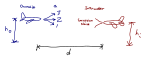
\includegraphics[width=0.7\textwidth]{unresponsive_acas.pdf}
\end{center}

\begin{itemize}
    \item The state space is 4-dimensional $\mathcal{S} = \mathbb{R}^4$, with each state consisting of $s=(h_o, \dot{h}_o, h_i, d)$ where $h_o$ is the ownship altitude in feet, $\dot{h}_o$ is the rate of climb in ft/min, $h_i$ is the intruder altitude in feet, and $d$ is the distance between the aircraft in feet.
    \item The action space is $\mathcal{A}=\{-1500, 0, 1500\}$ and represents the change in rate of climb. The possible rates of climb are $\dot{h}_o \in \{-3000, -1500, 0, 1500, 3000\}$
    \item A reward of -100 is received for a near-mid-air collision, defined as the aircraft passing within 500 vertical feet and 100 horizontal feet of each other. Any change in rate of climb yields a reward of -1.
    \item The rate of climb, $\dot{h}_o$ changes instantly when an action is applied. Then the following dynamics are used: $d' = d - 2\,v\,\Delta t$ where $v$ is the fixed horizontal velocity, $h_o' = h_o + \dot{h}_o\,\Delta t$, and $h_i' = h_i + W_{\Delta t \sigma^2}$ where $W$ is the Wiener process\footnote{\url{https://en.wikipedia.org/wiki/Wiener_process}}. $\Delta t$ changes based on the discretization \texttt{n}.
\end{itemize}

\end{document}
